\label{sec:Res}
\section*{Results}

\subsection*{Constant environment and density-dependence}

We used the previously developed model in \citetext{Sandell et al. 2014, master's thesis} and simulated (see~\autoref{fig:dd}) a tree population for 150 years in constant environment, with and without density-dependence on $s_0$, to model a more realistic demography.

Indeed, density-dependence introduced a limit in the population (\autoref{fig:dd} right panel), as the number of mature and immature individuals seem to converge respectively to $18000$ and $10000$ individuals, while without density-dependence the population is exponentially growing.

Looking at the phenotype, we started from exactly the same starting point $z=116$ for phenotypic and genotypic values. Without density-dependence, the population quickly converge to the equilibrium phenotype ($\overline{z_{weak}}$ given by the approximation in~\autoref{eq:zweak}), $\overline{z_{weak}} = 166$ in this case. With density-dependence the equilibrium is shifted upward ($\overline{z_{weak, dd}} = 121.8$).

This shift is due to the decrease of $s_0$ in the density-dependent model, indeed because of the initial population $s_{0, dd} = 1.18 10^-3$ while $s_0 = 0.03$ without density-dependence. This difference, all else being equal, changes the equilibrium of $\overline{z_{weak}}$. With a lower seed survival, the equilibrium is shifted towards $\theta_s$, i.e. the survival optimum for immature, because it compensates to maintain the demographic equilibrium (growth rate = 1).

Within the density-dependent model the mean immature phenotype $\overline{z_I}$ converge quicker than the mean mature phenotype $\overline{z_M}$ to the equilibrium. It is because of stage-structured nature of our model, the mature stage is a combination of individuals that lived for around 40 generations (given our life-cycle), it buffers adaptation. To change $\overline{z_M}$, the individual have first to be closer to $\overline{z_{weak}}$ than to survive for a certain number of years and become mature. While the newborns of the given generation are already closer to the equilibrium.

\begin{figure}[ht!]
	\centering
	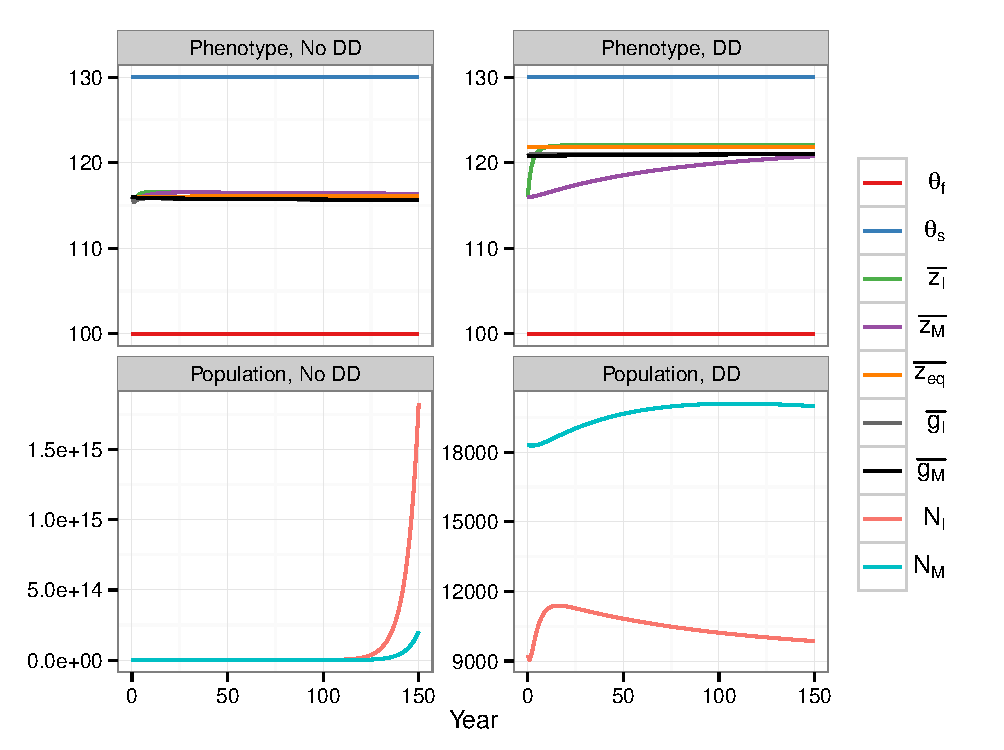
\includegraphics[scale=1]{Figures/DDphenopop.pdf}
	\caption{\textbf{Effect of density-dependence on phenotypes and populations}. \textbf{Left panel}: Phenotype variations in population ($\overline{z_I}, \overline{z_M}$) with their corresponding genotypic values ($\overline{g_I}, \overline{g_M}$) all starting from $z = 166$, and the approximation given by \autoref{eq:zweak}; \textbf{right panel}: demography, number of immature individuals ($N_I$, red), number of mature individuals ($N_M$, blue). Starting from Stable-Stage Distribution (SSD) in constant environment, note the logarithmic scale used.}
	\label{fig:dd}
\end{figure}

\subsection*{Fluctuating optimums}

To mimic a more realistic environment we made the optimums fluctuate, with various correlations between them. We simulated three populations using the same random seed. We only vary correlations between noises.

Explain in the text correlation of $z_{I}$ with $\theta_{s}(t)$

\begin{figure}[ht!]
	\centering
	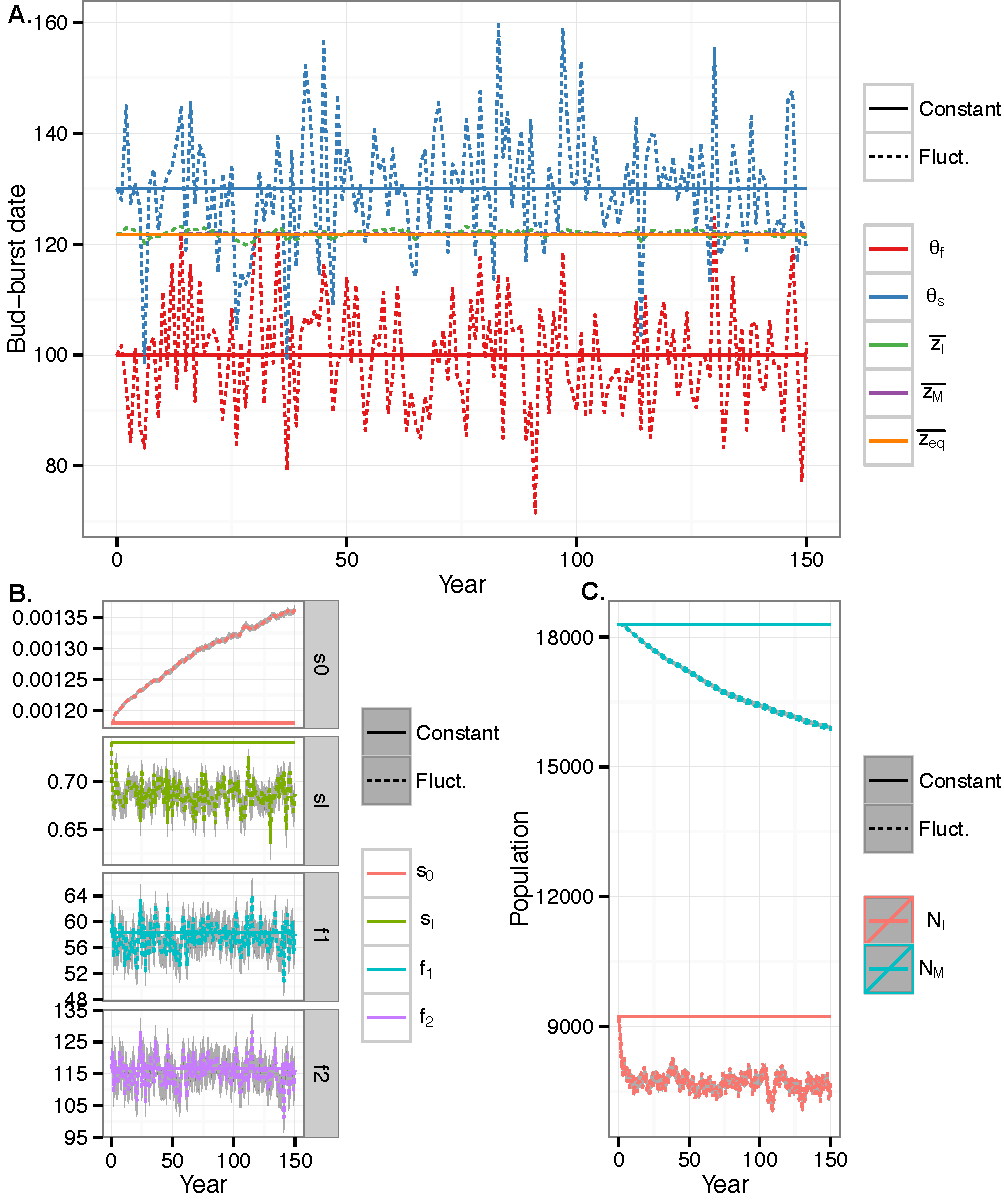
\includegraphics[scale=1]{Figures/PhenoLHTwithCorr.pdf}
	\caption{\textbf{Effect of the correlation of fluctuations on phenotypes and life-history traits}. Correlation coefficient $\rho_{N}$ values of noises are indicated at the the top of each column. Phenotype and approximations are shown in julian days, $\overline{z_\epsilon}$ is the approximation from \autoref{eq:zfluct}. Mean fecundities are in number of seeds produced. The two bottom rows are survival rates, the top one is $\overline{s_I}$ the mean survival of immature individuals, the bottom one is $s_0$ the rate of survival and germination of seeds (see~\nameref{sec:M&M}).}
	\label{fig:corr}
\end{figure}

\subsection*{Trend in the environment}

\begin{figure}[ht!]
	\centering
	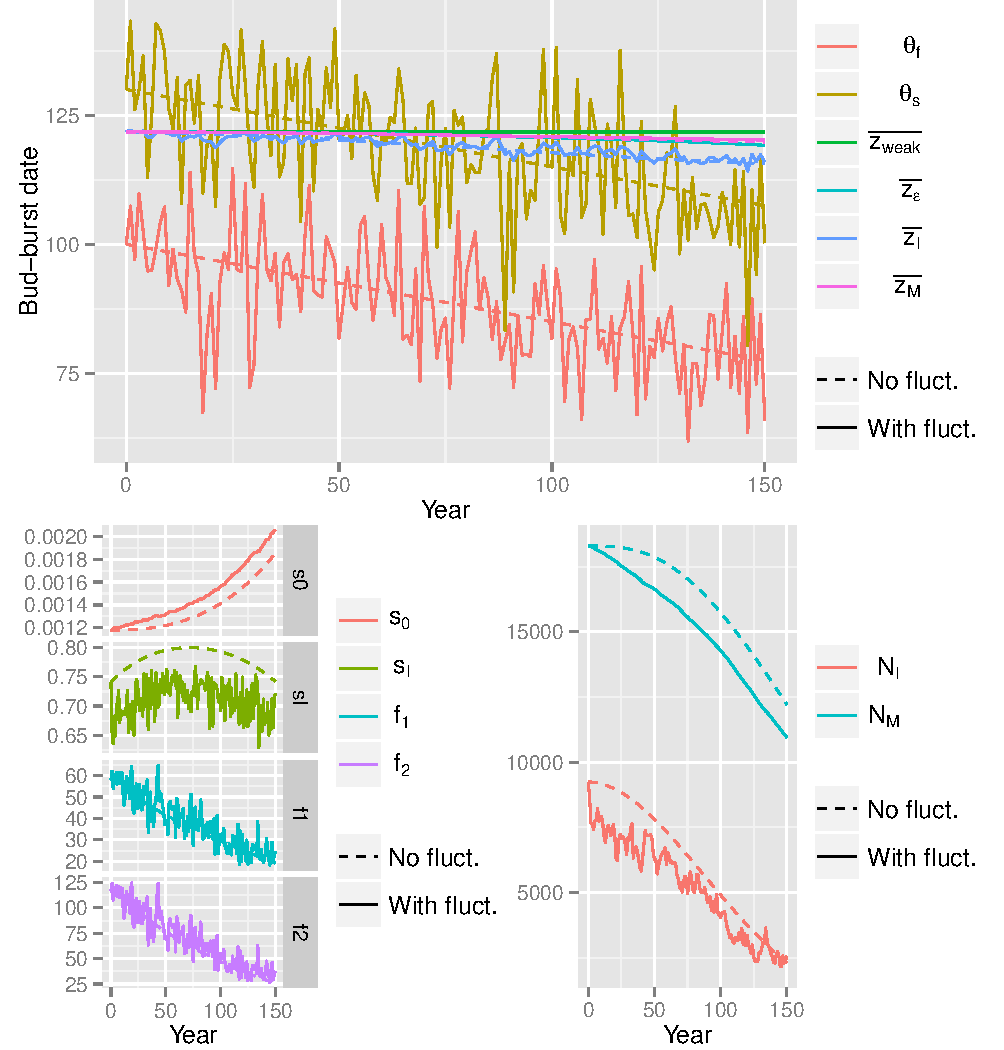
\includegraphics[scale=1]{Figures/Trend.pdf}
	\caption{\textbf{Mixed influences of trend and fluctuations on the population}. \textbf{Top panel}: Phenotype evolution with and without fluctuations; \textbf{Bottom:} (\textbf{Left}) Life-History Traits evolution depending on fluctuations, (\textbf{Right}) demography.}
	\label{fig:thetaf}
\end{figure}

Decreasing optimums through time to mimic the advance in phenology with climate change.

\textbf{Figure:} Trend 2 panels with and without fluctuations, simulations results phenotype/time (with and without DD)

\subsection*{Estimation of the fluctuations}

\begin{figure}[ht!]
	\centering
	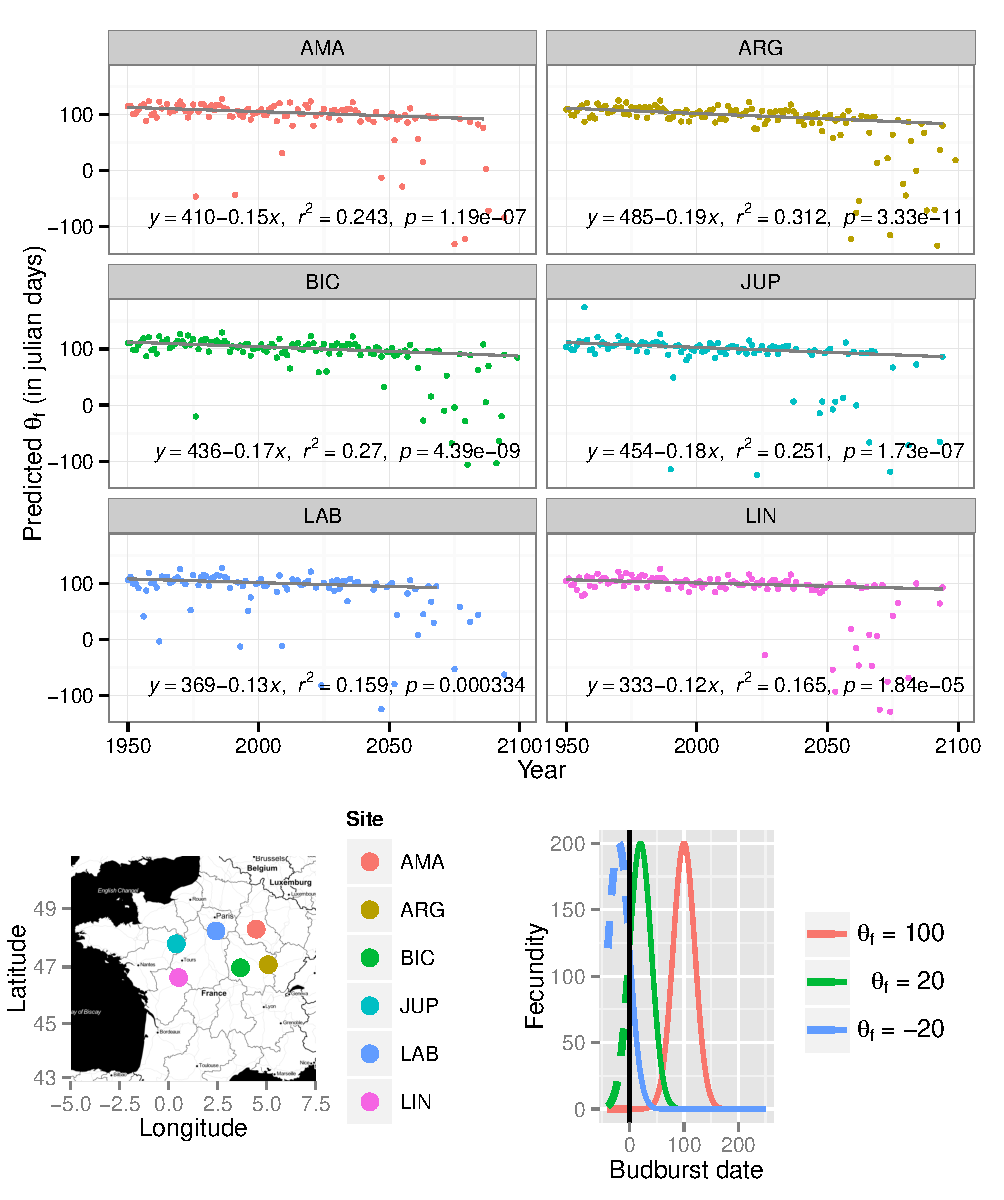
\includegraphics[scale=1]{Figures/optsmaps.pdf}
	\caption{\textbf{$\theta_{f}$ estimations from PHENOFIT data}. Top 3 rows: estimations of $\theta_f$ for each study site see \nameref{sec:M&M} for details. Bottom left panel: map of the study sites. Bottom right panel: Theoretical fecundity functions with parameters from~\autoref{tab:params} with values of $\theta_f$ equals to $100$, $20$ and $-20$, solid lines indicate achievable phenotype, dashed lines show theoretical curves but unreachable phenotypes.}
	\label{fig:thetaf}
\end{figure}

From 6 localities (map \autoref{fig:thetaf} bottom left) of \textsc{PHENOFIT} data, we computed $\theta_f$ values at these locations (top 3 rows of \autoref{fig:thetaf}). For the 6 sites, predicted $\theta_f$ decrease with time, it is more precocious as time passes. This observation matches the advance of phenology observed in the literature because of climate change.

Over the general trend, we observe a small amplitude variation around 20 days, corresponding to year to year change in $\theta_f$ and some dramatic decreases in its values, sometimes reaching negative values (For example at BIC site in 1976). The frequency of these events increase with time as they become \"normal\" after 2050 for all sites. Note that those event are biased towards the decrease of $\theta_f$, as there is no equivalent dramatic increases.

The negative values of $\theta_f$ computed in \autoref{fig:thetaf}, may seem striking as there is no such thing as a negative bud-burst date! However, as bottom right panel of \autoref{fig:thetaf} shows, we can have negative value of $\theta_f$ and still have achievable phenotypes. And if $\theta_f$ is very negative for a given year (less than -100 in 2048 for LAB), it means that will be no reproduction this year.

We excluded those extreme events to estimate the trend in the variation of $\theta_f$ (see~\nameref{sec:M&M}). Using linear regression on $\theta_f$ with time, we found a rate of \SI{-0.15}{\day\per\year}, with normal residuals having a variance of \SI{93.1}{\day\squared} (data not shown, $R^2=0.2435$, $p=1.185e-07$, $F=32.5$ with $101$ d.f.).

We investigated to know if there was a break between years modeled from real data by \textsc{PHENOFIT} (before 2001) and years modeled using climate models with climate change included (from 2001). We performed the same regression as above, without taking apart the extreme values, for all sites, splitting the data before 2001 and from 2001. Taking all years, for each site.